\documentclass[]{article}
\usepackage[margin=.5in]{geometry} 
\usepackage{grid-system, graphicx}

\newcommand{\plotpath}[1]{{../plots_oberbayern/#1}.pdf}
\newcommand{\plotwidth}{.8\textwidth}
\newcommand{\plotrow}[2]{\begin{Row}
		\begin{Cell}{1}%
			\centering
			\includegraphics[width=\plotwidth]{\plotpath{#1}}%
		\end{Cell}%
		\begin{Cell}{1}%
			\if\relax\detokenize{#2}\relax
			\else
			\centering
			\includegraphics[width=\plotwidth]{\plotpath{#2}}%
			\fi
		\end{Cell}
	\end{Row}
}

\begin{document}

\begin{center}
	\Huge Engelsberg im Vergleich mit Gemeinden im Regierungsbezirk Oberbayern
\end{center}

\vfill

\section*{Erläuterungen}
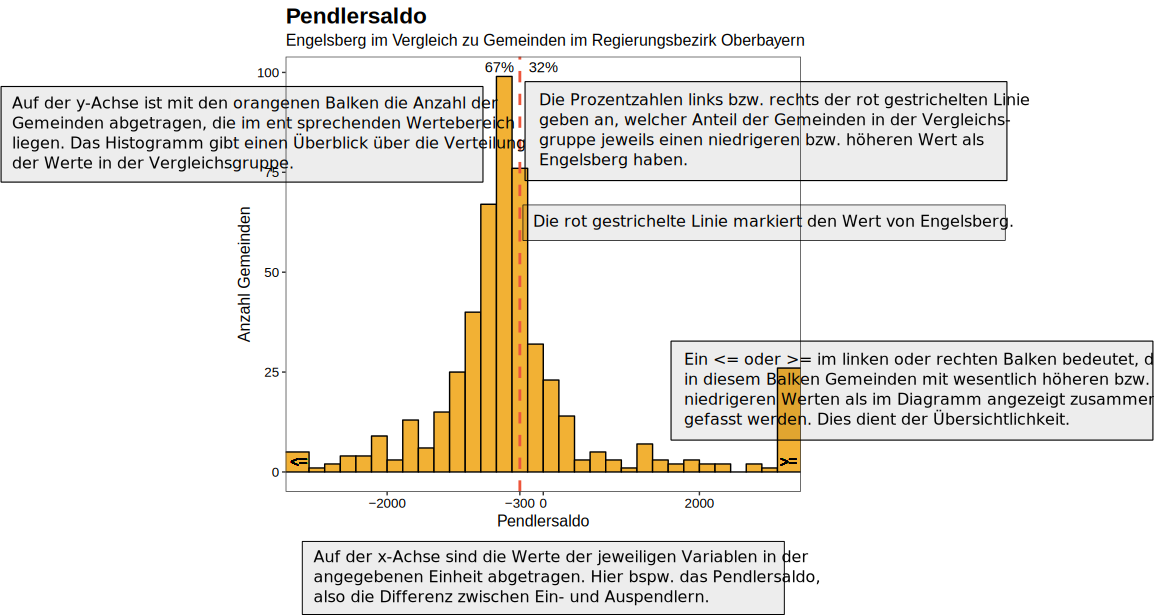
\includegraphics[width=\textwidth]{../plot_explanations}

\vfill

\section*{Bevölkerung}
	\plotrow{bevoelkerung.insgesamt}{bevoelkerung.je_km2}
	\plotrow{bevoelkerung.veraenderung.vs.1987}{bevoelkerung.veraenderung.vs.2011}
	\plotrow{bevoelkerung.bewegung.zugezogene}{bevoelkerung.bewegung.fortgezogene}
	\plotrow{bevoelkerung.bewegung.wanderungsgewinn}{altersstruktur}

\section*{Flächen}
	\plotrow{gebfreifl.rel}{betrfl.rel}
	\plotrow{landwfl.rel}{waldfl.rel}
	\plotrow{erholfl.rel}{}

\section*{Wohnen}
	\plotrow{bauwohn.bestand_wohnungen.insgesamt}{bauwohn.baugenehmigungen.wohnungen}

\section*{Kinderbetreuung und Bildung}
	\plotrow{bildung.kindertages.plaetze.pro100}{schueler.insg.rel}

\section*{Landwirtschaft und Umwelt}
	\plotrow{landforst.betriebe_von_flaeche_ha.insgesamt}{umwelt.wasser_pro_kopf_verbrauch}

\section*{Erwerb, Einkommen und Soziales}
	\plotrow{erwerb.sozialverspfl_beschaeftigte_am_arbeitsort.insgesamt}{erwerb.sozialverspfl_beschaeftigte_am_arbeitsort.darunter_einpendler.prozent}
	\plotrow{erwerb.sozialverspfl_beschaeftigte_am_wohnort.darunter_auspendler.prozent}{erwerb.pendlersaldo}
	\plotrow{lohneinksteuer.bruttolohn.je_arbeitnehmer}{lohneinksteuer.gesamtbetrag_einkuenfte.insgesamt}
	\plotrow{lohneinksteuer.gesamtbetrag_einkuenfte.je_steuerpfl}{sozialhilfe_empf.insg.rel}

\section*{Kommunale Finanzen}
	\plotrow{kommunale_finanzen.steuereinnahmen_insgesamt}{kommunale_finanzen.gemeindesteuereinnahmen.insgesamt}
	\plotrow{kommunale_finanzen.steuereinnahmekraft.je_einwohner}{kommunale_finanzen.realsteueraufbringungskraft}

\end{document}

%\begin{Row}
%	\begin{Cell}{1}
%		\includegraphics[width=\plotwidth]{\plotpath{}}
%	\end{Cell}
%	\begin{Cell}{1}
%		\includegraphics[width=\plotwidth]{\plotpath{}}
%	\end{Cell}
%\end{Row}
